\documentclass[11pt,a4paper]{article}
\usepackage[a4paper,top=2.0cm,bottom=2.0cm,left=2.1cm,right=2.1cm]{geometry}
\usepackage{setspace}
\usepackage{graphicx}
\usepackage{booktabs}
\usepackage{amsmath}
\usepackage[numbers]{natbib}
\onehalfspacing
\setlength{\parskip}{0pt}
\setlength{\parindent}{1.15em}
\pagestyle{plain}
\begin{document}

\begin{titlepage}
\centering
\vspace*{18mm}
{\Large Spatial Equity of Walking Access to Public Facilities and Public EV Chargers in Macao SAR\par}
\vspace{1.1em}
{\large CS482 Data Science\par}
\vspace{0.6em}
Group X\par
\vspace{1.5em}
{\normalsize Group member names\par}
\vspace{0.35em}
\rule{0.72\textwidth}{0.4pt}\par
\vspace{1.1em}
{\normalsize Student IDs\par}
\vspace{0.35em}
\rule{0.72\textwidth}{0.4pt}\par
\vspace{0.8em}
{\small Write each member's name and student ID on the lines above.\par This file does not fill them in.\par}
\vspace{1.3em}
{\normalsize Submission deadline:\par 15 December 2026, 23:59 Macao time\par}
\vspace{1.1em}
\begin{minipage}{0.9\textwidth}
\raggedright
\small
The cover, references, contribution statement, and AI declaration are outside the main-text page count. Every estimate in the main text is copied directly from the committed Phase A tables, refreshed Route A outputs (\texttt{outputs/metrics/phase\_b\_route\_a.json}), archived Colab Run 2 metrics (\texttt{outputs/metrics/phase\_b\_route\_b\_run2.json}), and exploratory tree outputs (\texttt{outputs/metrics/phase\_b\_exploratory\_trees.json}).
\end{minipage}
\end{titlepage}

\section{Introduction}
Residents of Macao do not share identical walking access to parks, public health centres, public libraries, bus stops, and public electric-vehicle (EV) chargers. This study addresses two descriptive questions. First, how unequal and spatially clustered is 10-minute and 15-minute pedestrian accessibility across populated H3 cells, and how is zone-level accessibility associated with the share of residents aged 65 or older after controlling for population density? Second, how accurately do spatial-block tabular models and graph neural networks capture the historical presence of public EV chargers from non-EV urban form and point-of-interest (POI) context?

Three hypotheses were pre-specified before inspecting estimates. \textbf{H1} posits that population-weighted accessibility is unequal and spatially clustered under false-discovery-rate (FDR) screening. \textbf{H2} compares the public EV charger Gini against parks, health centres, libraries, and bus stops on identical resampled cells. \textbf{H3} posits that, across the 23 terrestrial census zones, a higher elderly share is associated with lower accessibility once log population density is controlled. Planners at DSSCU and DSAT and local residents can use these maps to inspect thin walking coverage. All results are cross-sectional and correlational: they describe historical facility configurations, do not estimate causal siting effects, and do not prescribe where to build chargers.

\section{Data Collection and Preparation}
Population counts come from the DSEC 2021 census \citep{dsec2021}. Building polygons and statistical zones were read in native EPSG:8433 and transformed to EPSG:32649. Excluding the maritime zone yields terrestrial control totals of 681,293 residents and 82,751 residents aged 65 or older, allocated to H3 cells by area-weighted building intersection. The frozen grids contain 287 populated resolution-9 cells and 63 populated resolution-8 cells nested inside 23 terrestrial zones and 7 official parishes (including Taipa).

Public EV chargers come from the CEM station map API \citep{cem2026}. Coordinates are corrected for Macao's bounding box, and capacity equals distinct charger identifiers; station 9488798 has empty connector metadata and uses an imputed capacity of 12.0 from published pile counts. Parks, health centres, libraries, and bus stops are whitelist-filtered against official SSM, library, and IAM directories and cross-checked with OpenStreetMap \citep{osm2026} using 25 m cross-source deduplication only (preserving opposite bus poles). The cleaned layer has 240 parks, 11 health centres, 15 libraries, 587 bus stops, and 85 public EV stations. Pedestrian travel times are computed on the Geofabrik Macau OpenStreetMap walk graph \citep{osm2026} at 4.5 km/h with no slope impedance and no walkable cross-harbour link, keeping the Peninsula and the islands as separate components.

Five geographic blocks (seed 42) are frozen for all classifiers, holding 56 charger-present cells (prevalence 0.1951): three Peninsula blocks (29, 29, and 32 cells; 16, 11, and 14 positives) and two Island blocks (99 and 98 cells; 9 and 6 positives). Model inputs are strictly the 11 non-EV columns in \texttt{feature\_manifest.json} (population, elderly share, built form, and distances to LRT and bus). Coordinates, EV counts/capacity, POI text as numeric columns, and all \texttt{acc10\_}, \texttt{acc15\_}, and \texttt{lisa\_} columns are excluded. Text inputs for Route B are regex-stripped of multilingual EV and charging tokens before encoding.

\section{Methods}
Pedestrian accessibility is measured by Gaussian two-step floating catchment area (2SFCA) scores at 10-minute and 15-minute thresholds \citep{luo2003,dai2010}. To prevent extreme small-population sliver polygons on Coloane from compressing urban variation, the four-facility composite applies \(\log(1 + a / \mathrm{median}_{+}(a))\) to each traditional facility before min--max scaling to \([0,1]\) and equal averaging. Inequality uses population-weighted Gini and additively decomposed Theil T (within and between parishes, with \(0\ln 0 = 0\)) with 2,000-draw bootstraps (seed 42). Spatial clustering uses island-safe \(k=4\) nearest neighbours, global Moran's I, and two-sided local indicators of spatial association (LISA) with 999 permutations and Benjamini--Hochberg FDR \citep{anselin1995,bh1995}.

H2 uses paired bootstraps of Gini differences on identical resampled cells with Holm adjustment across the four traditional facilities. H3 is fit at the zone level (\(N=23\), using population-weighted centroids for zone 2SFCA) so building-allocated cells are not treated as independent replicates. Ordinary least squares with HC3 standard errors (small-sample \(t_{20}\) inference and exact Gaussian AIC), spatial error maximum likelihood (SEM-ML, residual Moran's I evaluated on spatially filtered errors \(e_{\mathrm{filtered}}\)), and spatial lag maximum likelihood (SLM-ML) are reported side by side under primary \(k=4\) weights and a bridge-augmented queen sensitivity matrix; diagnostic \(p\)-values never drop a model. Scale sensitivity compares resolution-8 and resolution-9 indices (MAUP).

Phase A classifiers evaluate a constant prior, L2 logistic regression, and random forest under the five frozen spatial blocks, fitting scalers and hyperparameter grids strictly inside training blocks. Primary classification metrics are five-fold mean ROC-AUC, PR-AUC, and top-20\% hit rate (recall inside the highest \(\lceil 0.20 n\rceil\) scores).

\section{Extension: Deep Learning Module}
Phase B evaluates graph neural networks on the frozen 988 directed 10-minute walk edges weighted by inverse walk time (\(w = 1/\mathrm{walk\_time\_min}\), normalized strictly by the training-edge mean). \textbf{Route A} trains three from-scratch networks over 10 seeds (42--51): two-layer residual \texttt{GATv2Conv} \citep{brody2022} (\texttt{edge\_dim=1}, 1,063,425 parameters), two-layer residual \texttt{TransformerConv} \citep{shi2021} (\texttt{edge\_dim=1}, 432,769 parameters), and an unweighted \texttt{GraphSAGE} capacity ablation \citep{hamilton2017} (5,149 parameters), using ELU activations, LayerNorm, Dropout 0.5, undirected DropEdge 0.3, and AdamW with cosine decay. Early stopping reads a fixed Peninsula inner block (block 2, or block 1 when fold 2 is held out), ensuring every fold retains both Peninsula and Island nodes (\(n_{\mathrm{loss}} = 156\text{--}226\)). Inductive training removes all test nodes and incident edges; inductive evaluation preserves \texttt{train}\(\to\)\texttt{train}, \texttt{train}\(\to\)\texttt{test}, and \texttt{test}\(\to\)\texttt{test} edges while forbidding \texttt{test}\(\to\)\texttt{train} so test features never enter training nodes. Transductive training keeps all edges while still masking test labels.

\textbf{Route B} fuses the 11 numeric features with 64-dimensional POI text representations from frozen \texttt{BAAI/bge-m3} (right-padded CLS token + train-only PCA), frozen \texttt{Qwen/Qwen3-Embedding-4B} (Matryoshka truncation + L2 normalization), and 4-bit NF4 QLoRA \citep{dettmers2023} (\(r=8\), \(\alpha=16\) on attention projections, 5,898,240 trainable parameters, logical encoder size 4.03B \(\le\) 5B). Archived Colab Run 2 (\texttt{phase\_b\_route\_b\_run2.json}, revisions {\ttfamily 5617a9f6} for BGE-M3 and {\ttfamily 5cf2132a} for Qwen) corrected Run 1's BGE left-padding bug, but forensic auditing revealed that Run 2 fit QLoRA on all four non-test blocks (including the inner validation block) and ran on pre-fix GNN splits, leading to premature epoch-1 stopping in 24/50 GATv2 LoRA fits and a noisy fold-2 batch loss increase (1.036 to 1.379). We therefore report Run 2 QLoRA with this explicit caveat and provide a leak-free Run 3 Colab pipeline (\texttt{scripts/colab\_phase\_b.py}, \texttt{notebooks/phase\_b\_colab.ipynb}) that restricts QLoRA strictly to \texttt{loss\_mask}, adds cosine LR with 4 shuffled epochs without replacement, fixes 4-bit logical parameter accounting, and preserves Run 1 and Run 2 archives. Outside the pre-specified plan, XGBoost, LightGBM, and HistGradientBoosting were evaluated strictly as exploratory tabular references.

\section{Results}
Figure 1 maps 15-minute log-scaled composite accessibility and BH-FDR LISA clusters across all 287 resolution-9 cells, showing clear urban gradients across the Peninsula, Taipa, Cotai, and Coloane. On resolution-9 cells at 15 minutes (Table 1), EV charger Gini is 0.4984 (95\% CI 0.4315--0.5566; Theil T 0.6706: 0.5085 within and 0.1622 between parishes), park Gini is 0.6115, health centres 0.4923, libraries 0.3249, bus stops 0.3876, and the composite index 0.1882 (Theil T 0.0673: 0.0487 within, 0.0185 between). At 10 minutes inequality rises across all surfaces (EV Gini 0.5850, park 0.6960, composite 0.3045). Although 35.54\% of populated cells have zero 15-minute EV access, those peripheral cells hold only 1.13\% of Macao's residents. Both primary surfaces are significantly clustered: composite Moran's I is 0.6061 (\(p=0.001\), 3 low-low and 9 high-high FDR cells) and EV Moran's I is 0.3450 (\(p=0.001\), 47 low-low and 1 high-high FDR cell). \textbf{H1 is supported for both composite and EV accessibility.}

For \textbf{H2} at 15 minutes, paired Gini differences show EV chargers are significantly more unequal than libraries (\(+0.1734\), CI \(+0.0867\) to \(+0.2512\), Holm \(p=0.0080\)) and bus stops (\(+0.1108\), CI \(+0.0479\) to \(+0.1658\), Holm \(p=0.0080\)), statistically indistinguishable from health centres (\(+0.0061\), CI \(-0.0815\) to \(+0.0936\), Holm \(p=0.8926\)), and less unequal than parks (\(-0.1132\), CI \(-0.1954\) to \(-0.0298\), Holm \(p=0.0550\); 10-min EV minus bus \(+0.1351\), Holm \(p=0.0080\)). Chargers are therefore not uniformly more unequal than every traditional facility. For \textbf{H3} on \(N=23\) zones (Table 1, Panel B), the 15-minute composite elderly-share coefficient is \(+1.9488\) under OLS-HC3 (95\% CI \(-0.6967\) to \(+4.5943\), \(p=0.1400\); log-density \(-0.0580\), \(p=0.0595\)), \(+1.9366\) under SEM-ML (\(p=0.0129\), filtered residual Moran \(0.0118\)), and \(+1.9635\) under SLM-ML (\(p=0.0111\)); park OLS-HC3 is \(+3.3187\) (\(p=0.7736\)), and bridge-queen weights yield matching signs. Because OLS-HC3 covers zero and spatial ML estimates are positive—opposite H3's negative direction—\textbf{H3 is not supported.} Under MAUP scaling, 15-minute composite Gini shifts modestly from 0.2293 (res-8) to 0.1882 (res-9, \(\Delta=-0.0412\)) and EV Gini from 0.4873 to 0.4984 (\(\Delta=+0.0110\)).

\begin{figure}[htbp]
\centering
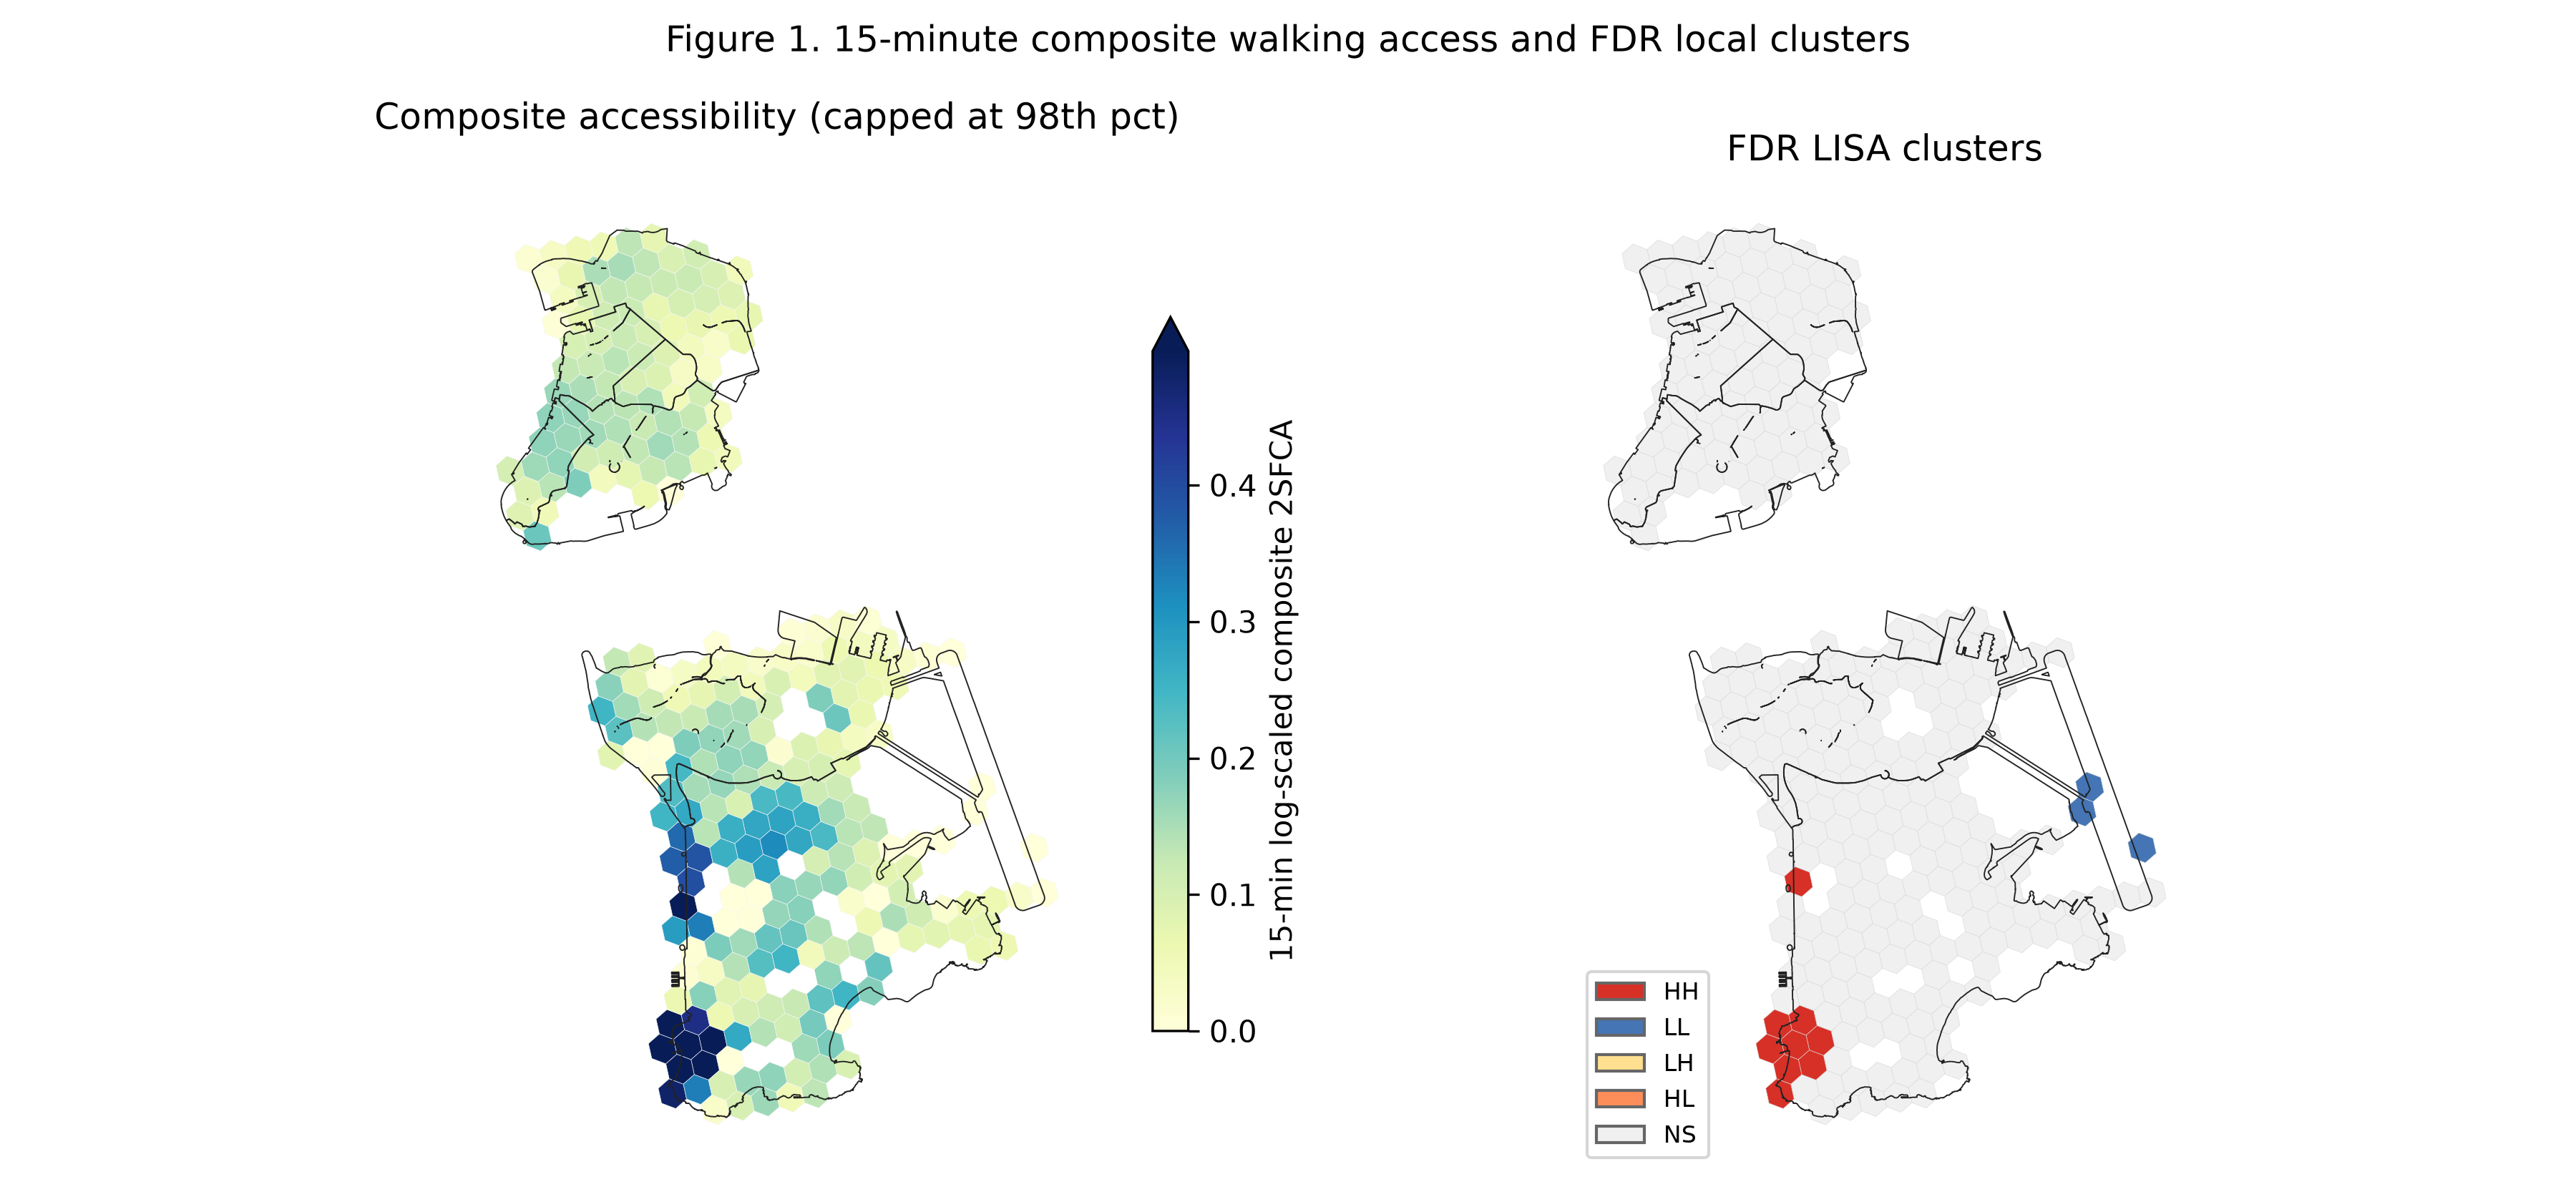
\includegraphics[width=0.96\textwidth,height=0.25\textheight,keepaspectratio]{../outputs/figures/fig1_accessibility_lisa.png}\\[3pt]
{\footnotesize\singlespacing \textbf{Figure 1.} Dual panel of 15-minute log-scaled composite accessibility (98th-percentile color cap) and two-sided BH-FDR LISA clusters across 287 resolution-9 cells. Colours describe historical coverage, not siting recommendations.}
\end{figure}

\begin{table}[htbp]
\centering
{\footnotesize\singlespacing
\renewcommand{\arraystretch}{0.95}
\textbf{Table 1.} Panel A: 15-minute population-weighted Gini (95\% bootstrap CI), Theil T within/between parish decomposition, Global Moran's I, and BH-FDR LISA cluster counts (res-9, \(N=287\)). Panel B: H3 15-minute composite elderly-share regression (\(N=23\), primary \(k=4\) weights).
\par\vspace{0.3em}
\setlength{\tabcolsep}{4.5pt}
\begin{tabular}{lrrrrrrr}
\toprule
Panel A: Facility (15 min) & Gini & 95\% CI & Theil T & Within & Between & Moran's I & LL / HH \\
\midrule
Park & 0.6115 & [0.5288, 0.6771] & 1.2912 & 0.9119 & 0.3793 & 0.5401 & 10 / 3 \\
Health centre & 0.4923 & [0.4124, 0.5655] & 0.5383 & 0.3437 & 0.1946 & 0.7493 & 0 / 9 \\
Library & 0.3249 & [0.2624, 0.3920] & 0.2766 & 0.1881 & 0.0885 & 0.7519 & 0 / 9 \\
Bus stop & 0.3876 & [0.3326, 0.4411] & 0.5972 & 0.4362 & 0.1610 & 0.0224 & 0 / 0 \\
EV charger & 0.4984 & [0.4315, 0.5566] & 0.6706 & 0.5085 & 0.1622 & 0.3450 & 47 / 1 \\
Composite (log-scaled) & 0.1882 & [0.1563, 0.2202] & 0.0673 & 0.0487 & 0.0185 & 0.6061 & 3 / 9 \\
\midrule
Panel B: H3 Composite (\(k=4\)) & \multicolumn{2}{r}{Elderly Coef} & \multicolumn{2}{r}{95\% CI} & \(p\)-value & AIC & Resid I \\
\midrule
OLS-HC3 (\(t_{20}\)) & \multicolumn{2}{r}{+1.9488} & \multicolumn{2}{r}{[\(-0.6967\), \(+4.5943\)]} & 0.1400 & \(-24.02\) & 0.0489 \\
SEM-ML (\(e_{\mathrm{filtered}}\)) & \multicolumn{2}{r}{+1.9366} & \multicolumn{2}{r}{[\(+0.4098\), \(+3.4634\)]} & 0.0129 & \(-24.17\) & 0.0118 \\
SLM-ML & \multicolumn{2}{r}{+1.9635} & \multicolumn{2}{r}{[\(+0.4482\), \(+3.4789\)]} & 0.0111 & \(-22.28\) & \(-0.0034\) \\
\bottomrule
\end{tabular}
}
\end{table}

Table 2 compares all charger-presence classifiers across the five frozen spatial blocks. Random forest leads all pre-specified and exploratory models (ROC-AUC \(0.773 \pm 0.111\), PR-AUC \(0.632 \pm 0.109\), top-20\% hit rate \(0.502 \pm 0.251\)), followed by exploratory XGBoost (\(0.741\)) and L2 logistic regression (\(0.736\)). On the refreshed, edge-weighted Route A GNNs with connected inductive evaluation, \texttt{TransformerConv} achieves \(0.705 \pm 0.032\) inductive / \(0.717 \pm 0.031\) transductive ROC-AUC, \texttt{GATv2} achieves \(0.679 \pm 0.019\) / \(0.689 \pm 0.013\), and \texttt{GraphSAGE} (5k) achieves \(0.652 \pm 0.056\) / \(0.658 \pm 0.020\); transductive scores consistently exceed inductive scores by \(+0.006\) to \(+0.012\) across all three architectures. In archived Colab Run 2, BGE-M3 fusion reaches \(0.728\) (inductive GATv2) and \(0.736\) (transductive TransformerConv), whereas Qwen-4B LoRA trails frozen Qwen under GATv2 (\(0.664\) vs \(0.708\)) and barely differs under TransformerConv (\(0.704\) vs \(0.692\) inductive; \(0.695\) vs \(0.696\) transductive), reflecting Run 2's validation-block leakage and small-sample variance. Using the pre-specified inductive GATv2 10-seed probability screen (\(\ge 0.7855\), 80th percentile among zero-charger cells) intersected with below-median 15-minute EV access (\(\le 0.000791\)) yields 13 field-check candidate cells recorded in \texttt{outputs/tables/phase\_b\_candidates.csv}.

\begin{table}[htbp]
\centering
{\footnotesize\singlespacing
\renewcommand{\arraystretch}{0.95}
\textbf{Table 2.} Spatial-block charger classification (ROC-AUC, PR-AUC, top-20\% hit rate). For single-seed tabular models (Phase A and exploratory trees), \(\pm\) is the 5-fold SD (ddof=0); for 10-seed GNNs, \(\pm\) is the 10-seed SD of the 5-fold mean (ddof=1)—the two dispersions are not directly interchangeable. Run 2 rows are archived pre-Run-3 Colab outputs.
\par\vspace{0.3em}
\setlength{\tabcolsep}{4.5pt}
\begin{tabular}{llccc}
\toprule
Model & Protocol / Stage & ROC-AUC & PR-AUC & Top-20\% Hit \\
\midrule
Constant prior & Phase A (CV) & \(0.500 \pm 0.000\) & \(0.304 \pm 0.195\) & \(0.190 \pm 0.167\) \\
Logistic regression & Phase A (CV) & \(0.736 \pm 0.094\) & \(0.520 \pm 0.114\) & \(0.388 \pm 0.189\) \\
Random forest (primary) & Phase A (CV) & \(0.773 \pm 0.111\) & \(0.632 \pm 0.109\) & \(0.502 \pm 0.251\) \\
\midrule
GATv2 (1.06M, weighted) & Route A, inductive & \(0.679 \pm 0.019\) & \(0.500 \pm 0.026\) & \(0.353 \pm 0.034\) \\
GATv2 (1.06M, weighted) & Route A, transductive & \(0.689 \pm 0.013\) & \(0.490 \pm 0.017\) & \(0.354 \pm 0.030\) \\
TransformerConv (0.43M) & Route A, inductive & \(0.705 \pm 0.032\) & \(0.523 \pm 0.041\) & \(0.386 \pm 0.053\) \\
TransformerConv (0.43M) & Route A, transductive & \(0.717 \pm 0.031\) & \(0.519 \pm 0.040\) & \(0.407 \pm 0.050\) \\
GraphSAGE (5k ablation) & Route A, inductive & \(0.652 \pm 0.056\) & \(0.474 \pm 0.067\) & \(0.336 \pm 0.066\) \\
GraphSAGE (5k ablation) & Route A, transductive & \(0.658 \pm 0.020\) & \(0.497 \pm 0.037\) & \(0.362 \pm 0.041\) \\
\midrule
BGE-M3 + GATv2 & Run 2 archive, ind. / trans. & \(0.728\) / \(0.680\) & \(0.559\) / \(0.470\) & \(0.421\) / \(0.372\) \\
BGE-M3 + Transformer & Run 2 archive, ind. / trans. & \(0.730\) / \(0.736\) & \(0.551\) / \(0.560\) & \(0.425\) / \(0.435\) \\
Frozen Qwen + GATv2 & Run 2 archive, ind. / trans. & \(0.708\) / \(0.667\) & \(0.494\) / \(0.442\) & \(0.398\) / \(0.320\) \\
Frozen Qwen + Transf. & Run 2 archive, ind. / trans. & \(0.692\) / \(0.696\) & \(0.473\) / \(0.488\) & \(0.386\) / \(0.378\) \\
LoRA Qwen + GATv2\(^*\) & Run 2 archive, ind. / trans. & \(0.664\) / \(0.681\) & \(0.510\) / \(0.491\) & \(0.367\) / \(0.376\) \\
LoRA Qwen + Transf.\(^*\) & Run 2 archive, ind. / trans. & \(0.704\) / \(0.695\) & \(0.514\) / \(0.531\) & \(0.403\) / \(0.377\) \\
\midrule
XGBoost & Exploratory (CV) & \(0.741 \pm 0.095\) & \(0.556 \pm 0.120\) & \(0.469 \pm 0.294\) \\
LightGBM & Exploratory (CV) & \(0.720 \pm 0.070\) & \(0.582 \pm 0.107\) & \(0.420 \pm 0.148\) \\
HistGradientBoosting & Exploratory (CV) & \(0.718 \pm 0.064\) & \(0.499 \pm 0.143\) & \(0.384 \pm 0.157\) \\
\bottomrule
\end{tabular}
\par\vspace{0.25em}
{\scriptsize \(^*\)Run 2 QLoRA fit included the inner validation block; leak-free Run 3 (\texttt{loss\_mask} only) is implemented in \texttt{scripts/colab\_phase\_b.py} for Colab GPU rerun.}
}
\end{table}

\section{Discussion}
Phase A answers H1--H3 without a siting rule. Both composite public-facility access and public EV charger access are unequal and spatially clustered under two-sided BH-FDR LISA (H1 supported), with within-parish disparity dominating total Theil inequality (72--76\%). Chargers are significantly more unequal than libraries and bus stops yet less unequal than parks (H2 mixed). At the zone scale (\(N=23\)), elderly share is not negatively associated with composite walking accessibility in OLS-HC3, SEM-ML, or SLM-ML (H3 not supported); older historic Peninsula zones coincide with denser traditional amenities.

Across all classification experiments, the tabular random forest (\(0.773\) fold-mean ROC-AUC) outperforms every from-scratch GNN, text-fused GNN, and exploratory boosted tree. This negative deep-learning result is informative: on a compact 287-node urban graph with 56 positives, two-hop neighborhood averaging oversmooths sharp cell-level commercial/residential built-form contrasts, and 0.4M--1.1M attention parameters over-parameterize 156--226 training cells. Consistent with this diagnosis, restoring connected inductive evaluation (\texttt{test}\(\to\)\texttt{test} edges) eliminated an earlier artifact where isolated test nodes inflated inductive GNNs above transductive ones, restoring the expected modest transductive advantage (\(+0.006\) to \(+0.012\) ROC-AUC). The 13 field-check candidates screened by inductive GATv2 (\texttt{phase\_b\_candidates.csv}) flag cells whose built form resembles historically charger-equipped cells despite low 15-minute EV coverage; they serve strictly as descriptive verification targets, not installation recommendations.

Four limitations bound interpretation. First, uniform area-weighted allocation inside building-group polygons cannot capture vertical density variation in Macao's high-rise districts. Second, facility capacity metadata are incomplete (unit weights for several amenities, imputed park areas, and imputed capacity 12.0 at station 9488798). Third, the walk network omits slope impedance, incomplete footbridges/overpasses, and cross-harbour links. Fourth, ecological fallacy applies: zone- and cell-level associations do not represent individual resident accessibility, and all estimates remain cross-sectional.

\clearpage
\bibliographystyle{plainnat}
\bibliography{references}

\section*{Contribution Statement}
This report is a group product. The geographic-data role covers DSEC census geometries, the CEM API feed, the OpenStreetMap walk network, and the frozen H3 grids. The spatial-statistics role covers Gaussian 2SFCA, Gini, Theil T, two-sided FDR LISA, and the zone-level OLS/SEM/SLM regressions. The machine-learning role covers the spatial-block baselines, the Phase B graph and text-attributed modules, and the exploratory trees. The remaining role covers the MAUP check, figures, numeric auditing, and assembly of this report. Group number, member names, and student IDs belong on the blank cover lines prior to Moodle submission. No member is credited with a causal siting claim.

\section*{AI Usage Declaration}
{\sloppy
AI coding assistants (Cursor and Antigravity) were used to plan, implement, audit, and revise the Phase A/B pipelines, unit/E2E tests, and LaTeX report drafts. Scientific-agent workflow guidance follows Kassis and coauthors \citep{kassis2026}. Assistants drafted code, tests, and prose, and performed forensic statistical/leakage audits, but were never permitted to fabricate metrics. Every number in this report is verified directly against committed CSV/JSON outputs (\texttt{h1\_inequality\_lisa.csv}, \texttt{h2\_gini\_diff\_bootstrap.csv}, \texttt{h3\_spatial\_regression.csv}, \texttt{maup\_r8\_vs\_r9.csv}, \texttt{phase\_a\_ml\_baselines.json}, \texttt{phase\_b\_route\_a.json}, \texttt{phase\_b\_route\_b\_run2.json}, and \texttt{phase\_b\_exploratory\_trees.json}). Archived Colab Run 1 and Run 2 outputs are preserved unchanged, with Run 2's QLoRA validation-leakage caveat explicitly documented alongside the leak-free Run 3 code prepared for Colab GPU execution.\par}

\end{document}
